\documentclass[border=3pt]{standalone}
% Preâmbulo compartilhado pelos diagramas TikZ da aula 9 de IHC (Princípios e Diretrizes)
\usepackage[T1]{fontenc}
\usepackage[utf8]{inputenc}
\usepackage{lmodern}
\usepackage{amsmath}
\usepackage{xcolor}
\usepackage{tikz}
\usetikzlibrary{arrows.meta,angles,quotes,decorations.pathmorphing,decorations.pathreplacing,calc,
                positioning,shapes.geometric,shapes.misc,backgrounds,fit,
                math}

% Paleta (mesma dos SVGs originais)
% Paleta da disciplina de IHC: acento roxo (#755099), da capa do livro.
% (o nome "dblue" é mantido para não alterar todos os diagramas)
\definecolor{dblue}{HTML}{755099}
\definecolor{dorange}{HTML}{B3541E}
\definecolor{dgreen}{HTML}{4A7C59}
\definecolor{dred}{HTML}{9C4B4B}
\definecolor{dcream}{HTML}{F4F1EA}
\definecolor{dshade}{HTML}{DDD7C9}

% Função gaussiana (não normalizada por padrão de escala visual)
\pgfmathdeclarefunction{gauss}{3}{%
  \pgfmathparse{1/(#3*sqrt(2*pi))*exp(-((#1-#2)^2)/(2*#3^2))}%
}

% Estilos comuns (prefixo d... para não colidir com chaves internas do pgf)
\tikzset{
  >={Stealth[length=2mm]},
  dguide/.style={gray!55, dashed, line width=0.4pt},
  daxis/.style={gray!60, line width=0.7pt, ->},
  dbody/.style={fill=black!3, draw=black!80, line width=1pt},
  dacc/.style={draw=dblue, line width=1pt},
  dlbl/.style={black!55, font=\small},
  dsub/.style={black!45, font=\footnotesize},
  dstate/.style={circle, draw=black!80, fill=dcream, line width=1pt,
                 minimum size=17mm, font=\large, inner sep=1pt},
  dobs/.style={circle, draw=black!80, fill=dshade, line width=1pt,
               minimum size=14mm, font=\large, inner sep=1pt},
  dbox/.style={rounded corners=2pt, draw=black!80, fill=dcream, line width=1pt,
               align=center, inner sep=6pt},
  dop/.style={circle, draw=black!80, fill=white, line width=1pt,
              minimum size=6mm, inner sep=0pt, font=\small},
  dtrans/.style={->, dblue, line width=1pt},
  dmeas/.style={->, dorange, line width=1pt},
  dcurve/.style={line width=1pt, dblue},
  dcurveb/.style={line width=1.4pt, dorange},
}

\begin{document}
\hyphenpenalty=10000 \exhyphenpenalty=10000 \tolerance=9999 \emergencystretch=3em
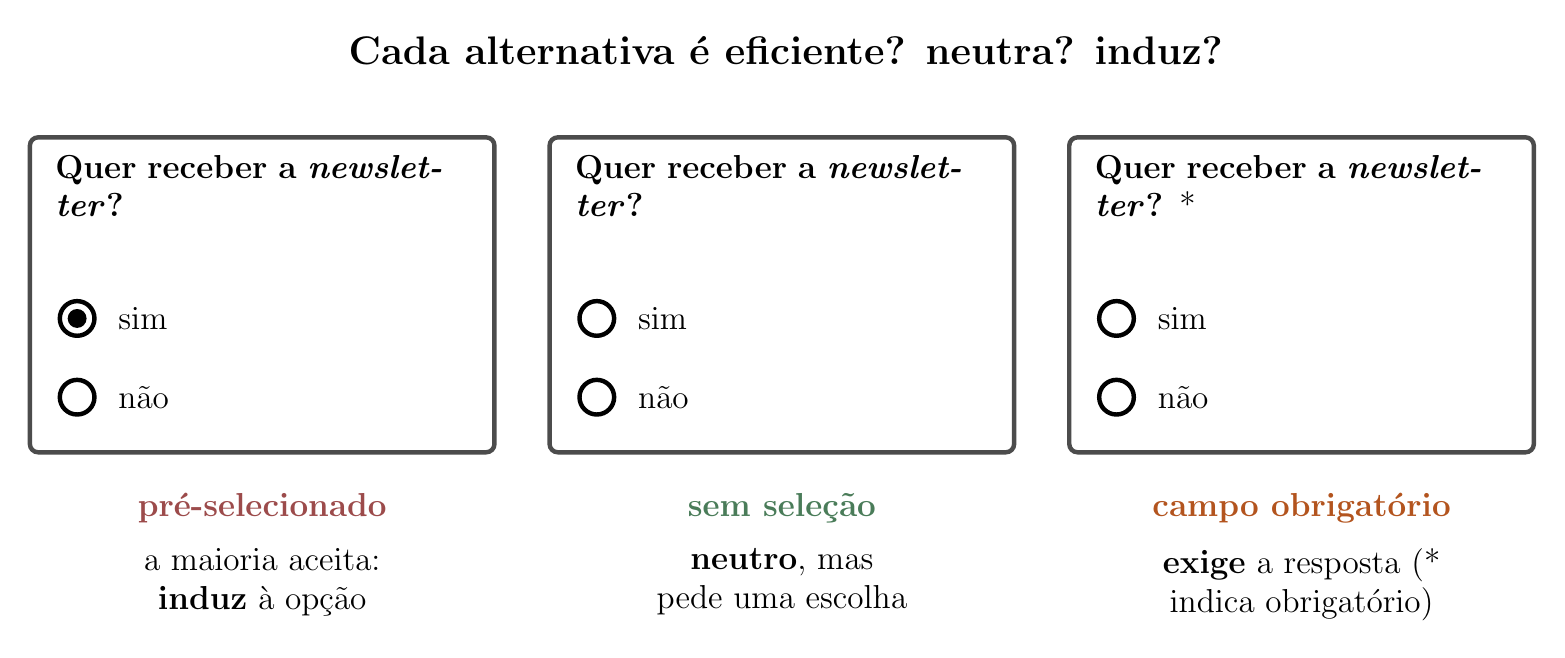
\begin{tikzpicture}[x=1cm,y=1cm]
\draw[draw=black!70, line width=1.6pt, fill=white, rounded corners=3pt] (0.0,3.2) rectangle (5.9,7.2);\node[font=\large, anchor=north west, text width=5.5cm] at (0.2,7.1) {\textbf{Quer receber a \emph{newsletter}?}};\draw[black, line width=1.6pt] (0.6,4.9) circle (0.22); \node[font=\large, anchor=west] at (1.0,4.9) {sim};\draw[black, line width=1.6pt] (0.6,3.9) circle (0.22); \node[font=\large, anchor=west] at (1.0,3.9) {não};\fill[black] (0.6,4.9) circle (0.12);\node[font=\large\bfseries, anchor=north] at (2.95,2.8) {\textcolor{dred}{pré-selecionado}};\node[font=\large, anchor=north, text width=5.6cm, align=center] at (2.95,2.1) {a maioria aceita: \textbf{induz} à opção};
\draw[draw=black!70, line width=1.6pt, fill=white, rounded corners=3pt] (6.6,3.2) rectangle (12.5,7.2);\node[font=\large, anchor=north west, text width=5.5cm] at (6.8,7.1) {\textbf{Quer receber a \emph{newsletter}?}};\draw[black, line width=1.6pt] (7.199999999999999,4.9) circle (0.22); \node[font=\large, anchor=west] at (7.6,4.9) {sim};\draw[black, line width=1.6pt] (7.199999999999999,3.9) circle (0.22); \node[font=\large, anchor=west] at (7.6,3.9) {não};\node[font=\large\bfseries, anchor=north] at (9.55,2.8) {\textcolor{dgreen}{sem seleção}};\node[font=\large, anchor=north, text width=5.6cm, align=center] at (9.55,2.1) {\textbf{neutro}, mas pede uma escolha};
\draw[draw=black!70, line width=1.6pt, fill=white, rounded corners=3pt] (13.2,3.2) rectangle (19.1,7.2);\node[font=\large, anchor=north west, text width=5.5cm] at (13.399999999999999,7.1) {\textbf{Quer receber a \emph{newsletter}?} *};\draw[black, line width=1.6pt] (13.799999999999999,4.9) circle (0.22); \node[font=\large, anchor=west] at (14.2,4.9) {sim};\draw[black, line width=1.6pt] (13.799999999999999,3.9) circle (0.22); \node[font=\large, anchor=west] at (14.2,3.9) {não};\node[font=\large\bfseries, anchor=north] at (16.15,2.8) {\textcolor{dorange}{campo obrigatório}};\node[font=\large, anchor=north, text width=5.6cm, align=center] at (16.15,2.1) {\textbf{exige} a resposta (* indica obrigatório)};
\node[font=\Large\bfseries] at (9.6,8.3) {Cada alternativa é eficiente? neutra? induz?};
\end{tikzpicture}
\end{document}
